\documentclass[11pt]{article}
\usepackage[margin=0.85in]{geometry}
\usepackage{mathptmx}
\usepackage[T1]{fontenc}
\usepackage{microtype}
\usepackage{amsmath, amssymb}
\usepackage{tabularx}
\usepackage{graphicx}
\usepackage{booktabs}
\usepackage{array}
\usepackage{xcolor}
\usepackage{listings}
\usepackage{enumitem}
\usepackage[hypcap=false]{caption}
\usepackage[hidelinks]{hyperref}

% --------------------------------------------------------------------------------------------
% Open, Readable Typography & Spacing
% --------------------------------------------------------------------------------------------
\linespread{1.08}
\setlength{\parskip}{0.45em}
\setlength{\parindent}{0pt}
\renewcommand{\arraystretch}{1.26}

\definecolor{codebg}{rgb}{0.975, 0.978, 0.985}
\definecolor{codecomment}{rgb}{0.22, 0.48, 0.32}
\definecolor{codekeyword}{rgb}{0.05, 0.22, 0.65}
\definecolor{codenumbers}{rgb}{0.52, 0.52, 0.52}
\definecolor{codestring}{rgb}{0.68, 0.12, 0.12}
\definecolor{accentblue}{rgb}{0.10, 0.32, 0.55}

\lstdefinestyle{logstyle}{
    backgroundcolor=\color{codebg},
    basicstyle=\ttfamily\footnotesize,
    breaklines=true,
    numbers=none,
    frame=single,
    rulecolor=\color{black!18},
    xleftmargin=0.6em,
    framexleftmargin=0.6em,
    aboveskip=6pt,
    belowskip=8pt
}
\lstset{style=logstyle}

\setlist[itemize]{leftmargin=1.4em, itemsep=0.25em, topsep=0.22em}
\setlist[enumerate]{leftmargin=1.5em, itemsep=0.30em, topsep=0.22em}
\captionsetup{font=small, labelfont=bf, skip=6pt}

\newcommand{\partheader}[1]{%
    \vspace{0.9em}%
    {\noindent\fontsize{13.5}{16}\selectfont\textbf{\color{accentblue}#1}\par}%
    \vspace{0.2em}\hrule\vspace{0.65em}%
}
\newcommand{\subhead}[1]{\vspace{0.55em}\noindent\textbf{\large #1}\par\vspace{0.22em}}

\begin{document}
\emergencystretch=1.8em

% ============================================================================================
% TITLE PAGE
% ============================================================================================
\begin{titlepage}
\begin{center}
    \vspace*{0.6cm}
    
\includegraphics[width=0.26\textwidth]{VNIT_logo.jpg}\\[1.0cm]

    {\large \textbf{Group Members}}\\[0.3cm]
    \begin{tabular}{l c l}
        Student 1: Gaurav Acharya & --- & [MT26MCS024] \\
        Student 2: Sandeep & --- & [MT26MCS032]
    \end{tabular}

    \vspace{0.85cm}

    {\large \textbf{Course \& Faculty Guide}}\\[0.25cm]
    CSP502 Software Lab-I --- M.Tech.\ CSE W26\\
    Visvesvaraya National Institute of Technology (VNIT), Nagpur\\
    Faculty Guide: Dr.\ A.\ S.\ Mokhade

    \vspace{0.85cm}

    {\large \textbf{Lab Exercise Title}}\\[0.25cm]
    {\Large \textbf{Resource-Aware, Fault-Tolerant and Priority-Based Event Processing in Go}}

    \vspace{0.8cm}

   
    \vspace{4cm}
    \small
    \begin{tabular}{ll}
        \toprule
        \textbf{Environment} & \textbf{Measured Specification} \\
        \midrule
        Go Toolchain & \texttt{go1.27.4-X:nodwarf5 linux/amd64} \\
        Hardware / OS & 12th Gen Intel Core i7-12650H (16 logical CPUs), Linux \\
        \texttt{GOMAXPROCS} & 16 (oversubscribed batch test: $W=32$) \\
        Datasets & Lab~4A logs (1k, 10k, 100k, 100k-variant; seed 42) + 18-line fixture \\
        \bottomrule
    \end{tabular}
\end{center}
\end{titlepage}

% ============================================================================================
% PART A
% ============================================================================================
\partheader{Part A --- Independent Reasoning and Design}
\textbf{Dated Design Record:} Frozen \texttt{2026-11-25T14:00:00+05:30} (\path{docs/partA_design_record.md}).

\subhead{A1. Claim Classification}
\begin{table}[htbp]
\centering
\caption{Classification of Scheduling, Concurrency, and Retry Claims.}
\footnotesize
\begin{tabularx}{\textwidth}{@{} >{\raggedright\arraybackslash}p{4.3cm} >{\raggedright\arraybackslash}p{2.0cm} >{\raggedright\arraybackslash}X @{}}
\toprule
\textbf{Claim} & \textbf{Verdict} & \textbf{Technical Justification} \\
\midrule
(i) Priority queues always improve service quality. & \textbf{Unjustified} & Priority scheduling favors \texttt{LOGIN\_FAILED} at the expense of normal events, causing normal-class starvation under high-priority pressure. \\
(ii) More workers eliminate overload. & \textbf{Unjustified} & When arrival rate exceeds sustainable capacity ($\lambda > \mu_{\max}$), extra workers add context-switch and lock contention without raising $\mu_{\max}$. \\
(iii) Retries are harmless. & \textbf{Unjustified} & Unbudgeted retries amplify load ($\lambda_{\text{eff}} = \lambda(1+r)$) during saturation and corrupt counts unless failed attempts commit zero side effects. \\
(iv) Faster average response implies better service for every class. & \textbf{Unjustified} & Aggregate means mask class-level starvation: 70\% fast high-priority events yield a low mean even while normal events stall for hundreds of milliseconds. \\
\bottomrule
\end{tabularx}
\end{table}

\subhead{A2. Data Structures, Complexity, Pipeline, and Predictions}
\begin{table}[htbp]
\centering
\caption{Queue Data-Structure Comparison ($K$ = queue capacity).}
\footnotesize
\begin{tabularx}{\textwidth}{@{} >{\raggedright\arraybackslash}p{3.4cm} l l >{\raggedright\arraybackslash}p{3.3cm} >{\raggedright\arraybackslash}X @{}}
\toprule
\textbf{Structure} & \textbf{Push / Pop} & \textbf{Memory} & \textbf{Tie-Breaking} & \textbf{Starvation Risk} \\
\midrule
Single FIFO Queue & $O(1)$ / $O(1)$ & $O(K)$ & Global arrival order & None \\
Binary Heap & $O(\log K)$ / $O(\log K)$ & $O(K)$ + seq & Needs \texttt{(prio, seq)} key & High for normal class \\
Separate Priority Queues (\texttt{highQ} + \texttt{normalQ}) & $O(1)$ / $O(1)$ & $O(K)$ split & Automatic FIFO per class & High unless paired with aging/weights \\
\bottomrule
\end{tabularx}
\end{table}

\begin{itemize}
    \item \textbf{Counting Complexity ($n$ events, $u$ unique IPs):} Repeated linear searches take $O(n \cdot u)$ expected and $O(n^2)$ worst-case ($u=\Theta(n)$). Go's hash-based \texttt{map[string]int} takes $O(n)$ expected ($O(1)$ amortized per lookup) and $O(u)$ space, with randomized per-map hash seeds mitigating collision worst cases.
    \item \textbf{Pipeline \& Ownership:} \texttt{Input} $\rightarrow$ \texttt{Validator} (assigns unique \texttt{EventID} $1..N$; counts malformed separately) $\rightarrow$ \texttt{Scheduler} (owns \texttt{highQ}/\texttt{normalQ} under \texttt{schedMu}) $\rightarrow$ \texttt{Workers} ($W$ goroutines) $\rightarrow$ \texttt{Ledger/Aggregator} (single mutex \texttt{aggMu} commits at most one terminal status per ID and updates counters only on \texttt{Successful}). Terminates cleanly when intake closes and workers drain queues.
    \item \textbf{Pre-Coding Predictions:} Skewed IPs improve map cache locality; D1/D4 bursts will starve normal events under strict priority; D2 slow tasks (5$\times$ cost) will cause HOL blocking in FIFO; reduced workers ($W$) cut $\mu_{\max}$ linearly. \textit{Success criteria:} exact accounting, 0 duplicates, post-burst recovery $\le 250$\,ms, and bounded normal wait ($\le 60$\,ms under Part~E).
\end{itemize}

% ============================================================================================
% PART B
% ============================================================================================
\newpage
\partheader{Part B --- Baseline Validation and Correctness}

All four Lab~4A logs (seed~42) and a hand-verified 18-line fixture (\path{datasets/hand_verified_fixture.log}: 2 malformed, 1 duplicate valid line, IP \texttt{10.10.10.50} with exactly 5 failures, \texttt{10.10.10.60} with 4 failures) were validated before benchmarking. Strictly checking 6 space-delimited fields catches 0.1\% malformed records (1, 10, 100, and 100 lines across the four datasets) and accounts for them separately.

\begin{table}[htbp]
\centering
\caption{Lab~4A Dataset Validation Summary (\texttt{data/validation/validation\_summary.csv}, seed~42).}
\scriptsize
\setlength{\tabcolsep}{4pt}
\begin{tabular}{@{}lccccccc@{}}
\toprule
\textbf{Dataset} & \textbf{Lines} & \textbf{Valid} & \textbf{Malf.} & \textbf{Dups} & \textbf{Users/IPs} & \textbf{Fail / FileAcc / Other} & \textbf{SHA-256} \\
\midrule
\texttt{small\_1k} & 1,000 & 999 & 1 & 10 & 92 / 55 & 161 / 169 / 669 & \texttt{ab98cdc41c3e} \\
\texttt{medium\_10k} & 10,000 & 9,990 & 10 & 100 & 100 / 55 & 1,640 / 1,808 / 6,542 & \texttt{abbb1dbc4151} \\
\texttt{large\_100k} & 100,000 & 99,900 & 100 & 1,000 & 100 / 55 & 16,616 / 17,566 / 65,718 & \texttt{8ef216d619ec} \\
\texttt{large\_var\_100k} & 100,000 & 99,900 & 100 & 1,000 & 100 / 55 & 16,285 / 17,991 / 65,624 & \texttt{52d991b24abf} \\
\bottomrule
\end{tabular}
\end{table}

\textbf{Fixture \& Race-Detector Verification:} Both \texttt{go test -count=1 -v ./...} and \texttt{go test -count=1 -race -v ./...} passed \textbf{5/5 tests} with 0 data races (\path{data/tests/race_test.log}). On the fixture, Sequential, FIFO, Priority, and Modified all flagged exactly \texttt{["10.10.10.50"]} and matched reference counts 100\%.

% ============================================================================================
% PART C
% ============================================================================================
\partheader{Part C --- Performance and Scheduling Investigation}

We implemented \textbf{Separate Priority Queues} (\texttt{highQ} + \texttt{normalQ}, $O(1)$ enqueue/dequeue, strict FIFO tie-breaking within each class) as the alternative to single FIFO. Parsing and trace setup were excluded from timed benchmarks ($5\,\mu\text{s}$ simulated work/event, 3 repetitions, median reported).

\begin{table}[htbp]
\centering
\caption{Fault-Free Batch Scaling on 100k Datasets (\texttt{data/batch/batch\_summary.csv}; Speedup / Efficiency shown; $W=32$ is oversubscribed).}
\scriptsize
\setlength{\tabcolsep}{3.8pt}
\begin{tabular}{@{}lccccccc@{}}
\toprule
\textbf{Dataset} & \textbf{Policy} & \textbf{$W=1$ (s)} & \textbf{$W=2$} & \textbf{$W=4$} & \textbf{$W=8$} & \textbf{$W=32$} & \textbf{Heap} \\
\midrule
\texttt{large\_100k} & Sequential & 0.5115 & --- & --- & --- & --- & 20.5\,MB \\
\texttt{large\_100k} & FIFO & 0.6316 (0.81$\times$) & 1.39$\times$ / 70\% & 2.28$\times$ / 57\% & \textbf{3.09$\times$} / 39\% & 2.82$\times$ / 8.8\% & 118.2\,MB \\
\texttt{large\_100k} & Priority & 0.6396 (0.80$\times$) & 1.39$\times$ / 70\% & 2.28$\times$ / 57\% & 2.66$\times$ / 33\% & 2.79$\times$ / 8.7\% & 117.5\,MB \\
\texttt{large\_var\_100k} & Sequential & 0.5129 & --- & --- & --- & --- & 20.6\,MB \\
\texttt{large\_var\_100k} & FIFO & 0.6350 (0.81$\times$) & 1.31$\times$ / 65\% & 2.23$\times$ / 56\% & 2.75$\times$ / 34\% & 2.74$\times$ / 8.6\% & 122.5\,MB \\
\texttt{large\_var\_100k} & Priority & 0.6386 (0.80$\times$) & 1.37$\times$ / 69\% & 2.19$\times$ / 55\% & \textbf{3.07$\times$} / 38\% & 2.76$\times$ / 8.6\% & 116.2\,MB \\
\bottomrule
\end{tabular}
\end{table}

\begin{figure}[htbp]
    \centering
    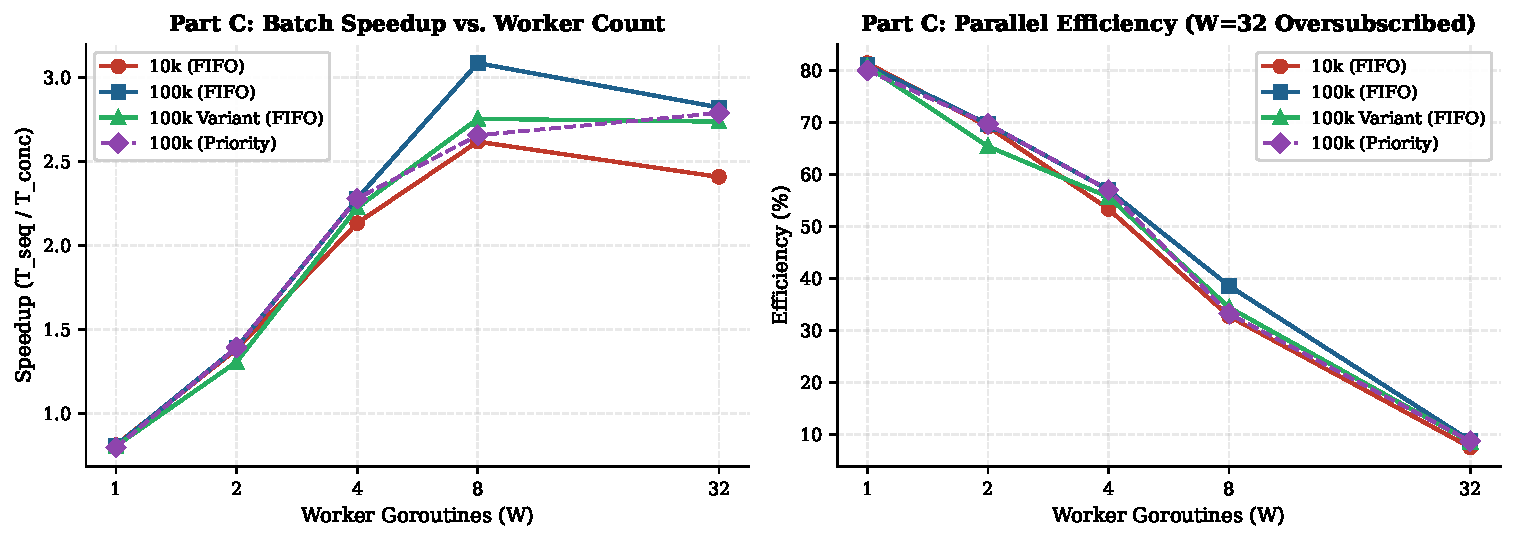
\includegraphics[width=0.95\textwidth]{figures/plot_partC_batch_scaling.pdf}
    \caption{Part~C batch speedup and parallel efficiency across worker counts ($W=1..32$). Speedup peaks near $W=8$ ($\sim 3.1\times$) due to shared scheduler/aggregator lock contention and plateaus/dips at oversubscribed $W=32$.}
\end{figure}

% ============================================================================================
% PART D
% ============================================================================================
\newpage
\partheader{Part D --- Controlled Disturbances ($W=4$, Unbounded Queue)}

Using identical deterministic 1,200-event paced replay traces (\path{configs/trace_D*.json}, nominal rate 950\,req/s, base cost 1.8\,ms), we evaluated D0--D4 on FIFO and Priority baselines before adding resilience mechanisms.

\begin{table}[htbp]
\centering
\caption{Part~D Baseline Disturbance Measurements (\texttt{data/disturbances/disturbances\_raw.csv}, $W=4$; FIFO vs.\ Priority).}
\scriptsize
\setlength{\tabcolsep}{2.6pt}
\begin{tabular}{@{}lccccccccc@{}}
\toprule
\textbf{Scenario} & \textbf{Succ.} & \textbf{Fail} & \textbf{PkQ} & \textbf{Thru.} & \textbf{High Med/p95 (ms)} & \textbf{Norm Med/p95 (ms)} & \textbf{MaxNW (ms)} & \textbf{Rec.\ (ms)} \\
\midrule
D0: Normal & 1200 / 1200 & 0 / 0 & 2 / 2 & 950 / 950 & 2.5/3.6 vs 2.5/3.6 & 2.5/3.5 vs 2.5/3.6 & 0.22 / 0.20 & --- \\
D1: Burst (3$\times$) & 1200 / 1200 & 0 / 0 & 190 / 190 & 1221 / 1221 & 36.7/119 vs \textbf{3.2/4.6} & 23.6/120 vs 25.6/135 & 127.3 / \textbf{141.8} & 339.1 / 338.9 \\
D2: Slow (10\% 5$\times$) & 1200 / 1200 & 0 / 0 & 11 / 12 & 946 / 945 & 3.4/13.0 vs 3.3/12.5 & 3.5/13.3 vs 3.4/13.9 & 10.6 / 14.0 & --- \\
D3: Fail (5\% 1st) & 1127 / 1127 & 73 / 73 & 2 / 2 & 891 / 891 & 2.4/3.5 vs 2.6/3.5 & 2.5/3.6 vs 2.4/3.5 & 0.20 / 0.23 & --- \\
D4: Prio 70\% & 1200 / 1200 & 0 / 0 & 2 / 2 & 946 / 946 & 2.5/3.6 vs 2.5/3.5 & 2.5/3.6 vs 2.5/3.5 & 0.18 / 0.19 & --- \\
\bottomrule
\end{tabular}
\end{table}

\begin{figure}[htbp]
    \centering
    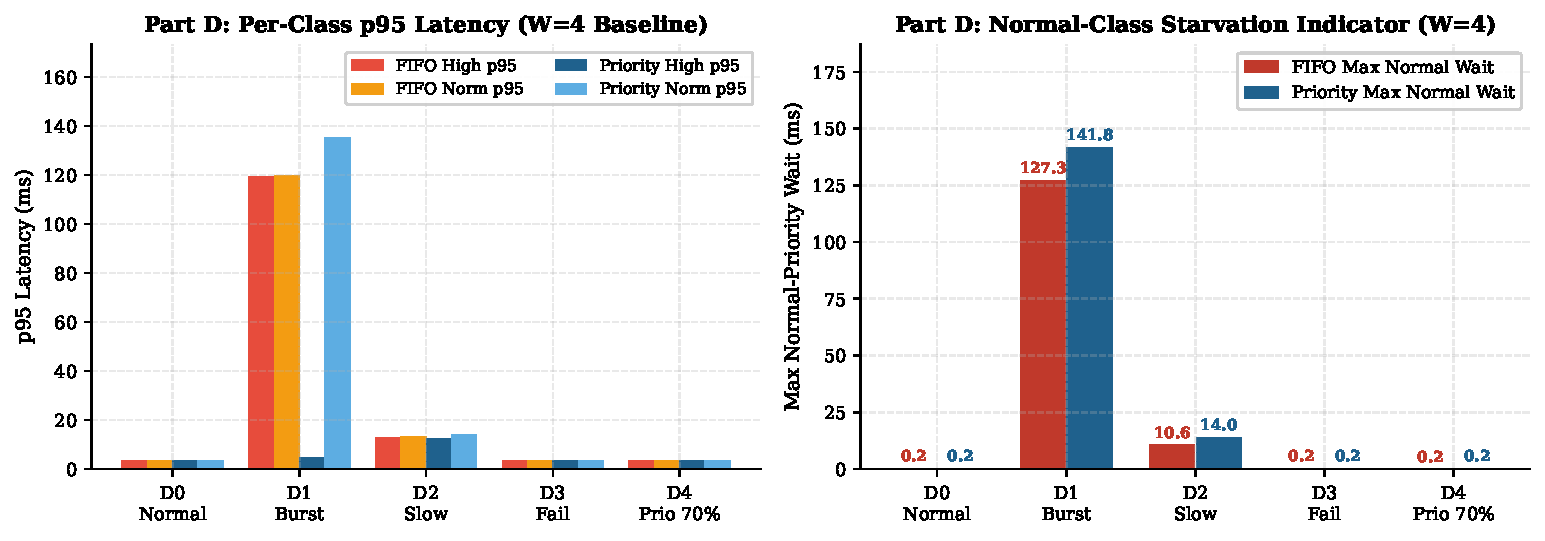
\includegraphics[width=0.95\textwidth]{figures/plot_partD_disturbances.pdf}
    \caption{Part~D baseline disturbances ($W=4$): under D1 Burst, Priority protects high-priority p95 (4.6\,ms vs.\ 119.4\,ms) while pushing normal p95 to 135.4\,ms and \texttt{MaxNormalWait} to 141.8\,ms. Under D3, 73 events fail permanently.}
\end{figure}

% ============================================================================================
% PART E
% ============================================================================================
\partheader{Part E --- Instructor-Issued Constraint and Redesign}
\textbf{Pre-Coding Change Record:} Frozen \texttt{2026-11-25T15:10:00+05:30} (\path{docs/partE_change_record.md}).\\
\textbf{New Operating Constraint:} Reduce capacity to \textbf{$W=2$ workers}, enforce a \textbf{strict queue limit $K=64$}, and keep \textbf{maximum normal-priority waiting time $\le 60$\,ms} across D0--D4.

\begin{itemize}
    \item \textbf{Invalidated Assumptions:} Unbounded queues ($PeakQ=190$ in D1) are no longer allowed; halving workers to $W=2$ makes 950\,req/s near-saturated, amplifying D2 HOL blocking and D4 normal-class starvation.
    \item \textbf{Mechanism 1 (Fairness --- Priority Aging + Weighted Cap):} Serve \texttt{highQ} by default, but promote \texttt{normalQ} whenever the head normal event waits $\ge 20$\,ms or after 4 consecutive high-priority dispatches.
    \item \textbf{Mechanism 2 (Overload/Failure --- Bounded Admission $K=64$ + Per-Task Timeout 15\,ms + Bounded Retry):} Fast-reject arrivals when full (\texttt{Rejected}), abort stalled tasks cleanly (\texttt{TimedOut}), and allow 1 retry (2 attempts max) for D3 transient failures with zero side effects on failed attempts and separate attempt counters.
\end{itemize}

% ============================================================================================
% PART F
% ============================================================================================
\newpage
\partheader{Part F --- Comparative Evaluation ($W=2, K=64$, 3 Repetitions)}

All 75 runs (5 policies $\times$ 5 scenarios $\times$ 3 repetitions) achieved \textbf{100\% accounting conservation} (\texttt{Generated = Successful + Failed + Rejected}), 0 duplicate outcomes, 0 missing IDs, $\Delta G = 0$ goroutines, and \textbf{exact match} against sequential replay of successful \texttt{EventID}s.

\begin{table}[htbp]
\centering
\caption{Part~F Comparative Means Across Original, Single-Mechanism, and Modified Designs ($W=2, K=64$).}
\scriptsize
\setlength{\tabcolsep}{3.0pt}
\begin{tabular}{@{}llccccccc@{}}
\toprule
\textbf{Scenario} & \textbf{Policy} & \textbf{Succ/Rej/Fail} & \textbf{Ret.} & \textbf{Thru.} & \textbf{High Med/p95} & \textbf{Norm Med/p95} & \textbf{MaxNW} & \textbf{Rec.\ (ms)} \\
\midrule
D0: Normal & Orig-FIFO & 1002 / 198 / 0 & 0 & 741 & 86.9 / 90.8 & 86.9 / 90.9 & 90.9 & N/A \\
D0: Normal & Orig-Prio & 1008 / 192 / 0 & 0 & 747 & \textbf{3.6 / 5.3} & 99.2 / 111.7 & 114.1 & N/A \\
D0: Normal & Modified-Full & 1003 / 197 / 0 & 0 & 743 & 375.5 / 468.1 & \textbf{24.8 / 35.6} & \textbf{36.6} & N/A \\
\midrule
D1: Burst & Orig-FIFO & 795 / 405 / 0 & 0 & 744 & 86.3 / 90.9 & 86.1 / 90.7 & 90.1 & 498.9 \\
D1: Burst & Orig-Prio & 792 / 408 / 0 & 0 & 740 & \textbf{3.6 / 5.5} & 99.8 / 110.6 & 112.6 & 502.7 \\
D1: Burst & Modified-Full & 779 / 421 / 0 & 0 & 727 & 375.5 / 458.0 & \textbf{25.1 / 43.1} & \textbf{43.4} & 503.9 \\
\midrule
D2: Slow & Orig-FIFO & 735 / 465 / 0 & 0 & 529 & 119.6 / 147.3 & 119.0 / 147.1 & 151.9 & N/A \\
D2: Slow & Orig-Prio & 743 / 457 / 0 & 0 & 539 & \textbf{4.5 / 14.6} & 138.4 / 161.0 & 164.8 & N/A \\
D2: Slow & Modified-Full & 757 / 443 / 0 & 0 & \textbf{549} & 483.4 / 673.4 & \textbf{37.1 / 85.4} & \textbf{89.3} & N/A \\
\midrule
D3: Fail & Orig-FIFO & 933 / 201 / 66 & 0 & 690 & 86.6 / 92.0 & 86.6 / 91.9 & 91.1 & N/A \\
D3: Fail & Orig-Prio & 947 / 190 / 63 & 0 & 700 & \textbf{3.6 / 5.6} & 99.4 / 110.8 & 113.5 & N/A \\
D3: Fail & Resilience-Only & 952 / 248 / \textbf{0} & 56.7 & \textbf{701} & 3.7 / 6.4 & 107.1 / 119.2 & 123.2 & N/A \\
D3: Fail & Modified-Full & 950 / 250 / \textbf{0} & 54.3 & 698 & 385.7 / 503.8 & \textbf{25.2 / 53.2} & \textbf{55.9} & N/A \\
\midrule
D4: Prio 70\% & Orig-FIFO & 1008 / 192 / 0 & 0 & 743 & 86.1 / 90.7 & 85.9 / 90.8 & 90.8 & N/A \\
D4: Prio 70\% & Orig-Prio & 1005 / 195 / 0 & 0 & 742 & \textbf{4.4 / 6.1} & 259.3 / 315.3 & 331.4 & N/A \\
D4: Prio 70\% & Fairness-Only & 1009 / 191 / 0 & 0 & 745 & 111.4 / 124.3 & \textbf{23.3 / 25.2} & \textbf{23.2} & N/A \\
D4: Prio 70\% & Modified-Full & 987 / 213 / 0 & 0 & 726 & 114.4 / 130.4 & \textbf{23.4 / 25.3} & \textbf{23.7} & N/A \\
\bottomrule
\end{tabular}
\end{table}

\begin{figure}[htbp]
    \centering
    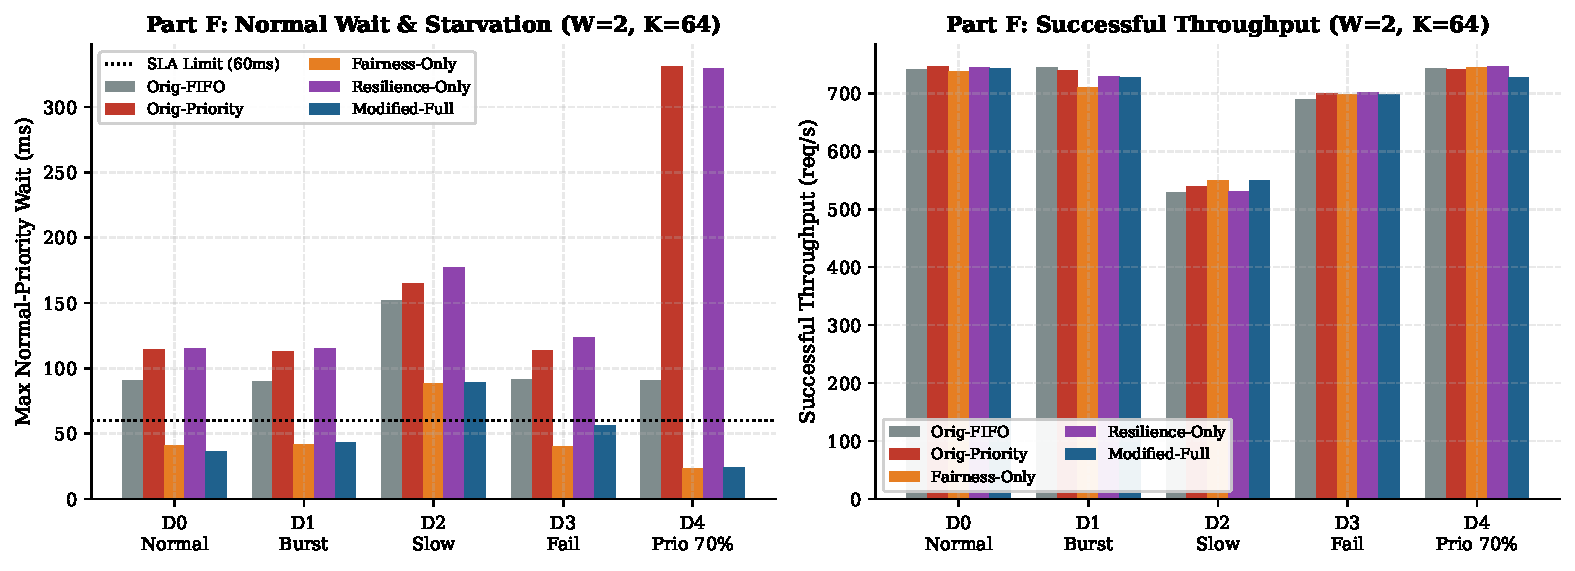
\includegraphics[width=0.95\textwidth]{figures/plot_partF_comparison.pdf}
    \caption{Part~F comparative evaluation ($W=2, K=64$): Fairness-Only and Modified-Full cut \texttt{MaxNormalWait} below the 60\,ms limit in D0, D1, D3, and D4 (23.7\,ms vs.\ 331.4\,ms in D4), while preserving throughput.}
\end{figure}

\textbf{Notes on Table Metrics:} \texttt{PeakQueueLen} was 64 across all $K=64$ runs; \texttt{TimedOut} and \texttt{Cancelled} were 0 in D0--D4 (since max slow cost $9\,\text{ms} < 15\,\text{ms}$ timeout and no external cancel was triggered; timeout/cancel paths are verified in \path{engine/engine_test.go}). Success-only latency equals accepted latency except in D3 where failed tasks finished in one attempt.

% ============================================================================================
% PART G
% ============================================================================================
\newpage
\partheader{Part G --- Engineering Judgment and Reflection}

\begin{enumerate}[itemsep=0.16em, topsep=0.12em]
    \item \textbf{Best data structure \& policy per workload:} Separate FIFO queues (\texttt{highQ}/\texttt{normalQ}) with $O(1)$ operations performed best overall. Under unconstrained $W=4$ normal load, strict Priority minimized high-priority p95 (4.6\,ms in D1) without starving normal tasks; under constrained $W=2$ and D4 (70\% high-priority), \textbf{Fairness-Only / Modified-Full} was essential to prevent 331\,ms normal starvation. No single policy wins everywhere because fairness protections inevitably add latency to high-priority events when capacity is saturated.
    \item \textbf{Priority vs.\ normal-class latency trade-off:} Yes. Under $W=2$ D4, strict Priority gave \texttt{HighMed} = 4.4\,ms while starving normal events to \texttt{NormMed} = 259.3\,ms (\texttt{MaxNormalWait} = 331.4\,ms). Aging fairness inverted this trade-off: \texttt{MaxNormalWait} dropped \textbf{14$\times$} to 23.7\,ms, at the cost of raising \texttt{HighMed} to 114.4\,ms.
    \item \textbf{Did retries improve completion or amplify overload?} Both. Under $W=2, K=64$ in D3, bounded retries eliminated all 63 permanent failures (raising class success rates from 94--95\% to \textbf{100\%}), but the 54.3 extra retry attempts consumed worker capacity and increased queue rejections from 190 to 250. Distinguishing \texttt{TotalAttempts} from unique \texttt{EventID}s prevents miscounting retries as throughput.
    \item \textbf{Contradicted pre-coding predictions:} We predicted 20\,ms aging would keep high-priority latency low during D0/D1 while only occasionally promoting normal tasks. Instead, because $W=2$ was saturated even at 950\,req/s, normal events aged past 20\,ms continuously and jumped ahead of \texttt{highQ}, pushing \texttt{HighMed} to 375.5\,ms in D0. A higher aging threshold (e.g., 45\,ms) or strict weighted ratio (e.g., 4:1 without aggressive 20\,ms promotion) is better when $W=2$ is saturated.
    \item \textbf{Recommended Operating Policy:} Deploy Separate Priority Queues with \textbf{$W=4$ workers}, \textbf{$K=64$ bounded queue} (explicit rejection above capacity), \textbf{4:1 weighted fairness + 45\,ms aging} (caps starvation without starving high-priority traffic under mild saturation), \textbf{1 bounded retry} for transient errors with zero side effects on failed attempts, and \textbf{15\,ms per-task timeout}. \textit{Limitations:} in-memory state is lost on crash, simulated sleeps do not model network/SQL locks, and $O(N)$ outcome ledgers need TTL eviction in long-lived daemons.
\end{enumerate}

\newpage
\subhead{AI Disclosure \& Member Contributions}
\textbf{AI-Tool Policy Disclosure:} Part~A and the Part~E pre-coding change response were completed independently without generative AI. For implementation, test scaffolding, plotting, and LaTeX formatting, AI assistance was used and independently verified by the group; \textbf{every number, log, and figure in this report comes from live local Go executions}.

\begin{itemize}
    \item \textbf{Gaurav Acharya [MT26MCS024]:} Part~A reasoning \& complexity analysis; \path{events/events.go} parser, validator, and replay trace builder; sequential reference and FIFO/Priority schedulers; automated fixture \& \texttt{-race} tests.
    \item \textbf{Sandeep [MT26MCS032]:} Part~E change record; aging fairness, bounded admission control, timeout \& retry mechanisms; \path{cmd/runner/main.go} benchmark harness; Python plotting suite; Parts~F--G evaluation.
\end{itemize}

\end{document}
